\section{Theorie}

\begin{flushleft}
    Der Aufbau des Franck-Hertz-Versuches, zu sehen in Abbildung \ref{Abbildung1}, besteht aus einem evakuierten Gefäß, in welchem sich ein Quecksilbertropfen befindet.
    Ein Teil des Quecksilbertröpfchen verdampft, wodurch sich ein Gleichgewichtsdampfdruck $\text{p}_{\text{sät}}$ einpendelt, welche nur von der Umgebungstemperatur T abhängig ist.
    Ebenso befindet sich ein Draht aus hochschmelzendem Metall in dem Glaskolben, der durch Gleichstrom bis auf Rotglut erhitzt wird.
    Der dabei auftretende glühelektrische Effekt sorgt dafür, dass sich die Elektronen aus dem Metall lösen und wie eine Wolke um den Draht legen.
    Gegenüberliegend von dem Glühdraht befindet sich eine netzförmige Elektrode, an welcher eine positive Gleichspannung $\text{U}_{\text{B}}$ angelegt wird.
    Beim Durchlaufen dieser Beschleunigungsstrecke erhalten die Elektronen die kinetische Energie 
\end{flushleft}

\begin{equation}
    \frac{\text{m}_{0} \cdot \text{v}^{2}_{\text{vor}}}{2} = e_{0}\,\text{U}_{\text{B}}\,. \label{1}
\end{equation}

\begin{flushleft}
    Dies gilt jedoch nur wenn die Elektronen zuvor die Geschwindigkeit $\text{v} = 0$ hatten. 
    Hinter dieser Beschleunigungselektrode befindet sich eine Auffängerelektrode, welche negativ geladen ist, damit die Elektronen abgebremst werden können.
\end{flushleft}

\begin{figure}[H]
    \centering
    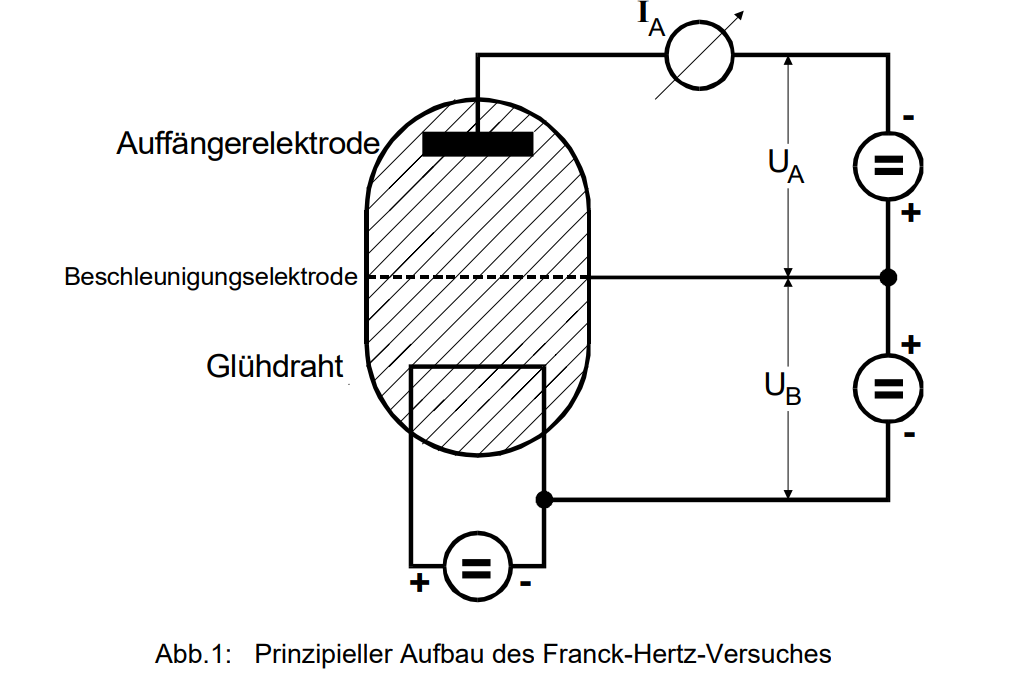
\includegraphics[height=75mm]{bilder/Ab1.png}
    \caption{Der Aufbau des Franck-Hertz-Versuches \cite{a1}. \label{Abbildung1}}
\end{figure}

\begin{align}
    \intertext{Elektronen dessen Geschwindigkeitkomponente $\text{v}_ {\text{z}}$ in  Feldrichtung die Ungleichung  }
    \frac{\text{m}_{0} \cdot \text{v}^{2}_{\text{z}}}{2} \geq e_{0}\,\text{U}_{\text{B}}\,, \label{2}
    \intertext{erfüllt, können gegen das Bremsfeld anlaufen und die Auffängerelektrode erreichen, wobei die anderen zur Beschleunigungselektrode zurückkehren.
    In dem Beschleunigungsraum kommt es zu verschiedenen Stößen zwischen den Elektronen und den Hg-Atomen.
    Bei geringer Energie der Elektronen treten nur elastische Stöße auf.
    Die Energieabgabe $\increment \text{E}$ des Elektrons wird aufgrund des großen Massenunterschiedes, zwischen dem Hg-Atom und dem Elektron, vernachlässigbar gering.
    Diese Energie beträgt} \notag
\end{align}

\begin{equation}
    \increment \text{E} = \frac{4\text{m}_{0}\, \text{M}}{(\text{m}_{0} + \text{M})^{2}} \cdot \text{E} \approx 1,1 \cdot 10^{-5}\,. \notag
\end{equation}

\begin{flushleft}
    wobei E die Energie des Elektrons ist.
    Trotz der vernachlässigbaren Energieverluste erfährt das Elektron bei dem Stoß eine Richtungsänderung.
    Wenn die Energie der Elektronen genauso groß oder größer als die Energiedifferenz $\text{E}_{1} - \text{E}_{0}$ ist, kommt es zu unelastischen Stößen zwischen den Elektronen und den Hg-Atomen.
    Auf diese wird der Energiebetrag der Energiedifferenz übertragen, wodurch diese angeregt werden.
    Unter Emission geht das Hg-Atom aus dem ersten angeregten Zustand wieder in den Grundzustand über und emittiert dabei einen Lichtquant mit der Energie
\end{flushleft}

\begin{equation}
    \text{h}\nu = \text{E}_{1} - \text{E}_{0}\,. \label{3}
\end{equation}

\begin{flushleft}
    Bei der Gegenfeldmethode wird der Strom an der Auffängerkathode beobachtet.
    Dabei wir die Beschleunigungsspannung kontinuierlich vergrößert.
    Wenn die Elektronen die Elektronenenergie $\text{E}_{1} - \text{E}_{0}$ erreichen, kommt es zu unelastischen Stößen und die Elektronen verlieren ihre Energie.
    Diese können dann folglich die Auffängerelektrode nicht mehr erreichen, was zu dem plötzlichen Abfall führt, welcher in Abbildung \ref{Abbildung2} zu sehen ist.
    Bei weiterer Steigerung der Beschleunigungsspannung sind die Elektronen in der Lage, nach dem Stoß erneut Energie aufzunehmen.
\end{flushleft}

\begin{figure}[H]
    \centering
    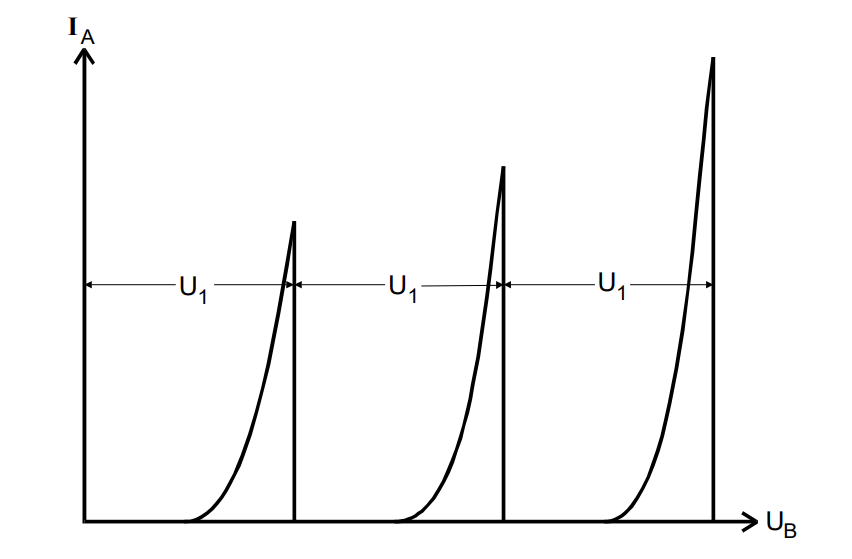
\includegraphics[height=60mm]{bilder/Ab2.png}
    \caption{ Auffängerstrom $\text{I}_{\text{A}}$ in Abhängigkeit von der Beschleunigungsspannung $\text{U}_{\text{B}}$ \cite{a1}.\label{Abbildung2} }
\end{figure}

\subsection{Störeinflüsse}

\begin{flushleft}
    Die beobachtete Franck-Hertz-Kurve ist idealisiert und weicht in einigen Punkten ab. 
    Diese werden in den folgenden Abteilen aufgelistet
\end{flushleft}

\subsubsection{Das Kontaktpotential}

\begin{align}
    \intertext{Da die Austrittsarbeit der Elektronen des Glühdrahtes und der Beschleunigungselektrode unterschiedlich sind, weicht das Beschleunigungspotential ebenso von der angelegten Beschleunigungsspannung $\text{U}_{\text{B}}$ ab.
    Dies führt dazu, dass für die effektive Brückenspannung durch}
    \text{U}_{\text{B, eff}} = \text{U}_{\text{B}} - \frac{1}{e_{0}}(\phi_{\text{B}} - \phi_{\text{G}}) \notag
    \intertext{ausgedrückt, wobei }
    \text{K} = \frac{1}{e_{0}}(\phi_{\text{B}} - \phi_{\text{G}}) \label{4}
    \intertext{das Kontaktpotential, um welches die Kurve auf der x-Achse verschoben, ist. } \notag
\end{align}


\subsubsection{Das Energie-Spektrum der Elektronen}

\begin{flushleft}
    Da die Leitungselektronen im Metall des Glühdrahtes bereits ein Energiespektrum besitzen, führt dies dazu, dass diese mit verschiedenen Anfangsgeschwindigkeiten aus dem Metall austreten.
    Dies sorgt dafür, dass unelastische Stöße über einen endlichen Einsatzbereich und nicht mehr bei einer genau definierten Beschleunigungsspannung vorhanden sind.
    Dadurch nähert sich die Franck-Hertz-Kurve flacher den Maxima an und fällt nicht abrupt auf null, sondern nähert sich stetig einem Minimum.
    Bei den elastischen Stößen kommt es durch eine Richtungssänderdung der Elektronen, zu einer Abflachung und Verbreiterung der Franck-Hertz-Kurve. 
\end{flushleft}


\subsubsection{Der Dampfdruck}

\begin{align}
    \intertext{Um eine ausreichend hohe Anzahl an Zusammenstößen zwischen Elektronen und Hg-Atomen zu erhalten, muss die mittlere freie Weglänge $\overline{\omega}$ kleiner sein als der Abstand zwischen der Beschleunigungselektrode und der Auffängerelektrode.
    Die mittlere frei Weglänge $\overline{\omega}$ beschreibt den Weg den Quecksilberatome zurücklegen bevor diese mit einem Elektron zusammenstoßen.
    Berechnet wird diese durch }
    \overline{\omega} = \frac{0,0029}{\text{p}_{\text{sät}}}\,. \label{5}
    \intertext{Der Sättigungsdruck $\text{p}_{\text{sät}}$ ist Temperaturabhängig und lässt sich durch  }
    \text{p}_{\text{sät}} = 5,5 \cdot 10^{7} \cdot \text{e}^{\frac{-6876}{\text{T}}} \label{6}
    \intertext{berechnen.
    Wenn der Sättigungsdruck zu groß wird, treten vermehrt elastische Stöße auf, was dazu führt, dass weniger Elektronen  die Auffängerelektrode erreichen. } \notag
\end{align}
